\section{Human Pose Estimation}
\label{section: background - human pose estimation}
% Explain what exactly human pose estimation is, and reference some papers discussing it. 
% Present the kinect and skeletal estimation, and \textbf{clearly specify} the \textbf{differences} between my \textit{arm location} estimation, and a \textit{full skeletal estimation}.

\textit{Human Pose Estimation} (\textbf{HPE}) is a broad term covering any system that tries to estimate the body position of people.
A well-known example of an HPE system is the Microsoft Kinect system, a camera-based movement tracker originally introduced for the Xbox game console.
Though HPE can cover a broad number of applications, many of them aim to construct a \textit{skeletal estimation}, a set of points that are indicative of the important joints on a human body, think of the head, shoulders, elbows, etc.
Microsoft Kinect, in particular, generates a skeletal estimate composed of 25 points, as depicted in \cref{fig:kinect_skeletal_estimate}, and is used as a source of ground truth for a number of other HPE systems.


\begin{figure}[h]
    \centering
    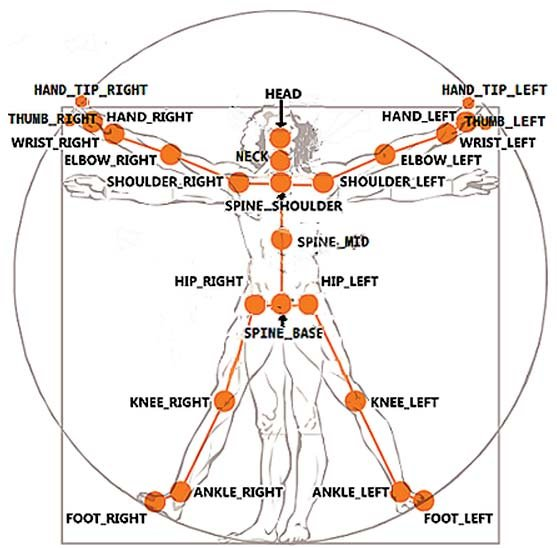
\includegraphics[width=0.5\linewidth]{figures/misc/The-skeleton-of-the-Kinect-v2-19.png}
    \caption{Kinect's 25-point skeletal estimation \cite{guffanti2020accuracy}}
    \label{fig:kinect_skeletal_estimate}
\end{figure}

\textbf{Something about arm angles vs skeletal estimate}.


HPE can be applied over various types of data, common methods are \textit{camera-based} HPE methods \cite{Lan2023visionbased}, \textit{wearable-based} HPE methods, or methods using other types of sensors, such as mmwave sensors.
Something most of these methods have in common thoug,h is their reliance on deep learning.
Many of the current state of the art systems, use deep learning to transform their video feed, or their pointcloud feed into skeletal estimations.